\documentclass{article}
\usepackage[letterpaper]{geometry}
\usepackage[utf8]{inputenc}
\usepackage{amsmath}
\usepackage{amssymb}
\usepackage{xcolor}
\usepackage{natbib}
\usepackage{graphicx}
\newcommand{\red}[1]{\textcolor{red}{#1}}
\newcommand{\mat}[1]{\boldsymbol{\mathsf{#1}}}
\renewcommand{\vec}[1]{\boldsymbol{\mathrm{#1}}}
\newcommand{\R}[1]{\mathbb{R}^{#1}}

\title{Learning Nonlinear Dynamics Using Kalman Smoothing}
\author{jmsh}
\date{October 2023}

\begin{document}

\maketitle

\abstract{Identifying Ordinary Differential Equations (ODEs) from measurement data requires both fitting the dynamics and assimilating, either implicitly or explicitly, the measurement data.  The Sparse Identification of Nonlinear Dynamics (SINDy) method thus involves a derivative estimation (and optionally, smoothing) step and a sparse regression on a library of candidate ODE terms.  Kalman smoothing is a classical framework for assimilating the measurement data whose noise behavior is well understood.  Previously, derivatives in SINDy and its python package, pysindy, had been estimated by finite difference, L1 total variation minimization, or local filters like Savitsky-Golay.  However, Kalman discovers ODEs that best recreate the essential dynamics in simulation, and when combined with hyperparameter optimization, requires the least amount of tuning.  We have incorporated Kalman smoothing into the existing pysindy architecture, allowing for rapid adoption of the method.  Using this standard engineering approach appears to be the most amenable to parameter selection and best at preserving problem structure in the presence of noise.  This is demonstrated on a number of dynamical systems.}

\section{Introduction}
The method of Sparse Identification of Nonlinear Dynamics, or SINDy, seeks to discover a differential equation governing an arbitrary, measured system.  The method takes as input some coordinate measurements over time, such as angles between molecular bonds \red{(Boninsegna article)} or a spatial field, such as wave heights \red{(Rudy article)}, and returns the best ordinary or partial differential equation (ODE or PDE) from a library.  However, the method struggles to accomodate significant measurement noise.  On the other hand, Kalman theory has a half-century history of assimilating noisy data to smooth a trajectory.  Its noise properties have been well studied. The paper integrates mature, well-established Kalman theory with emerging SINDy technology and generalized cross validation parameter selection.  It finds that the combination is competitive with other combinations of data smoothing and system identification, and has an advantage in preservation of problem structure and ease of parameter selection.

% \begin{itemize}
%     \item Model discovery in data science - bring power of kalman here (what about other methods: autoencoders, DMD, Koopman) (what for?) (All of physics specifying relationships among derivatives) (your job is to discovery derivatives, because derivatives give you the models. There's a lot more we can say, study, and understand about a system when we can identify relationships between derivatives.
%     \item SINDy - overview (2016 + )
%     \item Kalman overview (citing textbooks: Kalman is (a) Euler update, (b) Filter update with normal random variable, (c) MLE of Brownian motion, (d) best linear fit) engineering practice and design have used it for control, data assimilation is used as a workhorse tool in the real world e.g. weather.  Plus Auto KS  Include words from https://www.sciencedirect.com/science/article/pii/S0003267000838398 about comparison between SG and Kalman.  Include words from https://en.wikipedia.org/wiki/Local\_regression about comparison between SG and LOES.
%     \item What we do: marriage of kalman + SINDy (figure, hinted at in P1)
% \end{itemize}

When developing model discovery methods for physical systems, explainability takes on greater importance. A method that can identify relationships between coordinates and derivatives supports all the theorems of physics, such as spectral analysis, local and global stability, and variable time-stepping.  While other time-series data science techniques have emerged such as dynamic mode decomposition, recurrent neural nets, and autoencoders, such methods do not seek to search a function space.  Applying any physical constraints to them, such as PINN \red{cite this} requires wholly new derivations.  Few tools exist to analyze the discovered models' global or local properties other than exhaustive simulation.

SINDy does seek to establish relationships between derivatives. Emerging from \red{cite original paper}, all variants aim to discover a sparse symbolic representation of an autonomous or controlled system, $\dot x = f(x)$.  This form has allowed innovations in regression that follow common physics techniques, such as bounding a Lyapunov function in \red{cite Trapping}, enforcing linear stability in \red{cite StableLinearSR3}, and weak formulation in \red{cite WeakSINDy}.  Explicitly stochastic extensions also provide symbolic representation of variance in \red{cite Boninsegna} and handle PDE discretization in \red{cite Langevin Regression}.  This paper could be considered a simpler approach in a similar vein to these latter methods.

Kalman smoothing, which this paper adds to SINDy, has a long history of assimilating measurement data in time series.  From its debut in \red{cite Kalman-original}, engineering practice and design have used it for control and prediction across the real world, e.g. in radar systems, econometric variables, weather prediction, and more.  The family of Kalman methods encompasses both smoothing, after-the-fact techniques, and filtering, real-time updates, that derive from the same assumptions for distributions.  The Kalman smoother can be considered as a best-fit Euler update, the maximum likelihood estimator of Brownian motion, or as the best linear fit of an unknown system.  In the simplest invocation, the Kalman estimator's only parameter is the ratio of measurement noise to the process's underlying stochastic noise.  Fixing both of these parameters allows Kalman methods to identify the variance of the associated estimator.  Furthermore, much work exists to attempt to identify parameters purely from data, such as \red{cite Floris, Boyd/Barrett}.  These methods include their own parameters and are not guaranteed a solution, but are an improvement on the indeterminate nature of direct maximum likelihood or MAP likelihood.

This paper introduces Kalman smoothing as the derivative estimation step in SINDy in distinction with the L1 total variation minimization or Savitsky-Golay smoothers common in application. By introducing a continuous process loss for derivative estimation, it begins to reconcile the derivative estimation step to the symbolic regression step in a principled manner.  It also allows engineering applications to incorporate SINDy estimation with a familiar data assimilation technique whose noise properties are well understood.

Section two describes the individual methods of SINDy and Kalman smoothing, providing some literature review.  In section three, experiments demonstrate the advantages of incorporating Kalman with SINDy.  The paper concludes with avenues for future research in section four.

\section{Background}

\subsection{SINDy}
SINDy \red{(PNAS paper)} is a family of emerging methods for discovering the underlying dynamics of a system governed by unknown or partially-known \red{(SR3 paper)} differential equations.  It can handle PDEs as well as PDEs \red{(Rudy Paper)}, and has been used for protein folding \red{(Boninsegna paper)}, chemical reaction networks \red{(Forgot paper)}, plasma physics \red{(Kaptanoglu papers)}, and more.  Most invocations occur through the pysindy Python package, but innovations such as Langevin Regression \red{(Callaham)} or \red{(Rudy integration paper)} exist as independent code.

Given some variable of interest $\mat X$ and a library of functions $\mat \Theta$ (including spatial derivatives, when relevant) SINDy seeks to find the coefficients $\mat \Xi$ of the differential equation:

\begin{align}
    \label{eqn:sindy_ode}
    \dot X = \Xi\Theta(X)
\end{align}

To amplify:
\begin{align*}
    &\mat X \in \R{n \times m}\text{: system of $n$ coordinates at $m$ timepoints.}\\
    &\mat \Theta(X) \in \R{p \times m}\text{: library of $p$ functions evaluated at $m$ timepoints}\\
    &\mat \Xi \in \R{n \times p}\text{: coefficients for $n$ equations of $p$ functions}
\end{align*}
The function library written as a time-independent quantity refers to the collection $\mat \Theta = [\theta_1, \dots \theta_p]^T$, where $\theta_i: \R{n}\rightarrow\R{}$. Examples include the family of all degree-2 polynomials of $n$ inputs, mixed sines and cosines of certain requencies, or any user-specified family.

The method generally proceeds in two steps: 

\begin{enumerate}
    \item Estimate the time derivatives of the system ${\mat{\widehat{\dot X}}} = G(\mat X)$ for some smoothing function $G$
    \item Choosing a sparse regression method, solve the problem $\underset{\text{sparse } \mat \Xi}{\arg\min} \left\| \mat{\widehat{\dot{X}}} - \mat \Xi \mat \Theta(\mat X) \right\|^2$
\end{enumerate}
Different methods exist for applying sparsity including sequentially thresholding linear regression, a direct L-0 penalty \red{cite SR3}, an L-0 constraint \red{cite MIOSR}, and bayesian methods that include an explicit regularizer and provide a distribution like spike-slab priors \red{cite Hirsch, Mars}.  A trade-off SINDy faces is that while sparse regression techniques work better with orthogonal basis functions, ODE for most physical systems have terms that are not orthogonal, e.g. the Lorenz system.

This paper seeks to make SINDy more resilient to noise by taking a data assimilation approach.  It instead presents the Kalman SINDy steps
\begin{enumerate}
    \item Estimate the state and time derivatives of the system ${\mat{\widehat{\dot X}}}, \mat{\widehat X} = G(\mat X)$ where $G$ uses Kalman smoothing
    \item Choosing a sparse regression method, solve the problem $\underset{\text{sparse } \mat \Xi}{\arg\min} \left\| \mat{\widehat{\dot{X}}} - \mat \Xi \mat \Theta(\mat {\widehat X}) \right\|^2$
\end{enumerate}

\subsection{Kalman Smoothing}

Kalman theory is a group of optimal estimation techniques to assimilate measurement noise to a random process.  The theory can be use to filter new measurements in real-time use cases or smooth a complete trajectory of measurements.  While the processes this paper is concerned with are not random, in the first step of SINDy they are unknown, and so probabalistic language is appropriate.


In adding Kalman smoothing to SINDy, we introduce a distinction between the measurement variables and the state variables of the dynamical system in equation 
\ref{eqn:sindy_ode}.  As such, the inputs to the problem become $m$ time points of measurements of $k$ variables ($\mat Z\in \R{k\times m}$) and a linear transform from the state to the measurement variables $\mat H \in \R{n \times k}$ describing how the process is measured.

Measurement error is assumed to be normally distributed with $\mat H \mat X - \mat Z \sim \sigma_z \mathcal N(0, \mat R)$ where the covariance matrix $\mat R\in\R{k,k}$.  Measurement regimes where noise is autocorrelated or varies over time can be accomodated by flattening $\mat H \mat X - \mat Z$ and describing $\mat R\in\R{nk,nk}$.

Two parameters are required $\sigma_z$, the measurement noise standard deviation, and $\sigma_x$, the process velocity standard deviation per unit time.  If only state estimates, and not variances, are required, it suffices to use the ratio $\rho = (\sigma_z / \sigma_x)^2$.

Each process is assumed to have an independent, Brownian velocity.  This leads to Kalman smoothing estimator 
\begin{align}
    \underset{X, \dot X}{\arg\min}{\|\mat H \mat X - \mat Z\|_{\mat R^{-1}}}^2 + \rho {\|\mat G [\mat {\dot X}, \mat X]\|_{\mat Q^{-1}}}^2
\end{align}
Here, $\mat G$ is a linear transform to separate $[\mat{\dot X}, \mat X]$ into independent, mean-zero increments, and $\mat Q$ is the covariance of the Brownian process velocity $\mat{\dot X}$ and its integral, $\mat X$ over the increments.

In practice, rather than choosing $\rho$, this paper uses the generalized cross validation of (\red{Barrett and Boyd paper}) to choose $\rho$.  It chooses $\rho$ in order to minimize the loss on a witheld set of data.  While the algorithm described in that paper is not guaranteed to find a minimum, heuristic experience has shown that the longer the trajectory, the more likely their algorithm will succeed.  As the experiments in the next section use simulated data, this limitation is acceptable.

\begin{itemize}
    \item Figure: Graphics of SINDy
    \item Figure: graphics of kalman smoothing
    \item Anything on existing Kalman System Identification?
\end{itemize}

\section{Experiments}

Seven canonical dynamical systems have been simulated, comparing the results of SINDy with Kalman smoothing and the hyperparameter optimization of \red{cite Boyd/Barratt} in comparison with alternative smoothing methods: L-1 total variation minimization and Savitsky-Golay.  The latter smoothing methods have been modified to pass the not just the smoothed derivatives $\mat{\widehat{\dot X}}$, but also the smoothed position estimates $\mat {\widehat X}$ to the second step of SINDy.  This is to allow direct comparison of the methods themselves and remove idiosyncracies of their implementations in the derivative package.  They also each require a parameter: TV requires a coefficient for the L-1 regularizer and Savitsky-Golay requires a smoothing window.  These are gridsearched over a wide range, although it is worth noting that choosing the gridsearched optimum requires knowledge of the true system, in distinction to the method used for Kalman smoothing.  The authors have edited the pysindy and derivative packages to enable Kalman smoothing and hyperparameter optimizations.

THe authors utilize an ensemble optimizer for SINDy, pioneered in \red{cite Urban} to bag both library terms and data points.  The inner optimizer is MIOSR, published in \red{cite WesG} with the correct number of terms specified a priori.  Presenting SINDy with the known number of nonzero coefficients is an attempt to present a best case, where we can ameliorate any interaction between the smoothing method and sparse optimizer caused by optimizer parameters. 

Methods can be compared in several ways: by the coefficients of the equations they discover, by their accuracy in forecasting derivatives, and how well the discovered system recreates observed dynamics in simulation.  As \red{cite Gilpin} (probably) notes,  metrics for dynamical system discovery are less universally understandable.  The merit of a metric depends upon both the use case and whether the trajectory considered is one of importance.  For instance, in controls engineering, the local derivative and very short-term forecasting is the primary imperative.  On the other hand, for reduced-order PDE models, recreating larger-scale phenomena in simulation may be more important.  Finally, in high-dimensional network dynamics, the accuracy of identifying connectivity, as measured by coefficient F1 score, is most important.

\begin{table}
    \label{tab:parameterization}
\end{table}
As the coefficient metrics are the most straightforwards, and we compare methods by F1 score and Mean Absolute Error.  We also compare predictive and simulated accuracy over a test set with the same distributional parameters as the training set.  Experiment parameterization is displayed in table \ref{tab:parameterization}.  Table \ref{tab:results} shows the results on all metrics to compare smoothing methods across all ODEs.
\begin{table}
    \label{tab:results}
\end{table}


\begin{figure}
    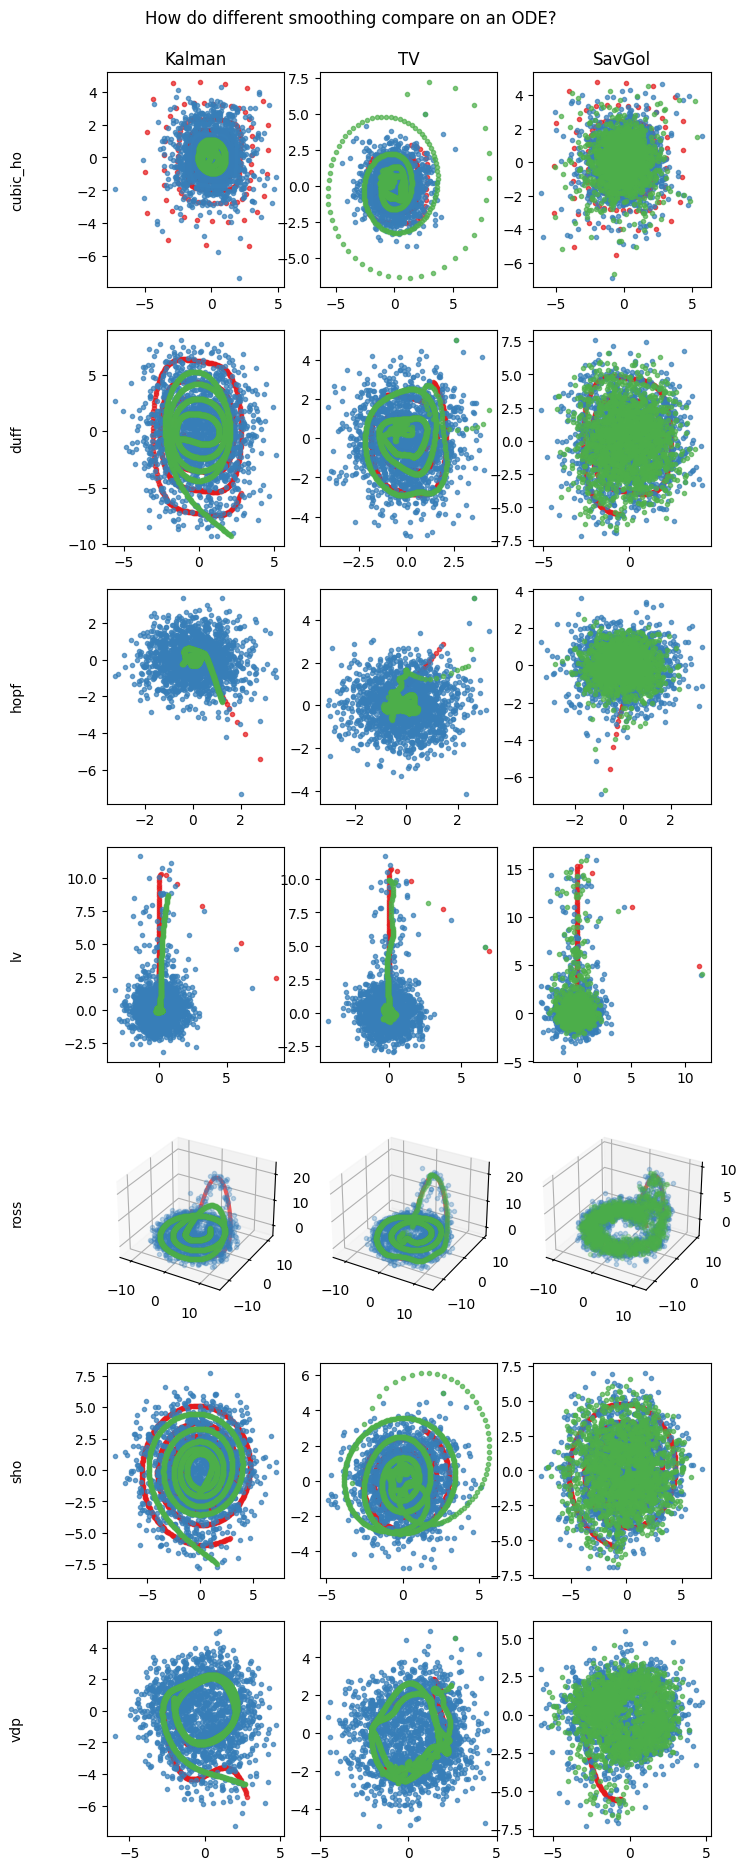
\includegraphics[height=\pdfpageheight]{images/summary_train}
\end{figure}
\begin{figure}
    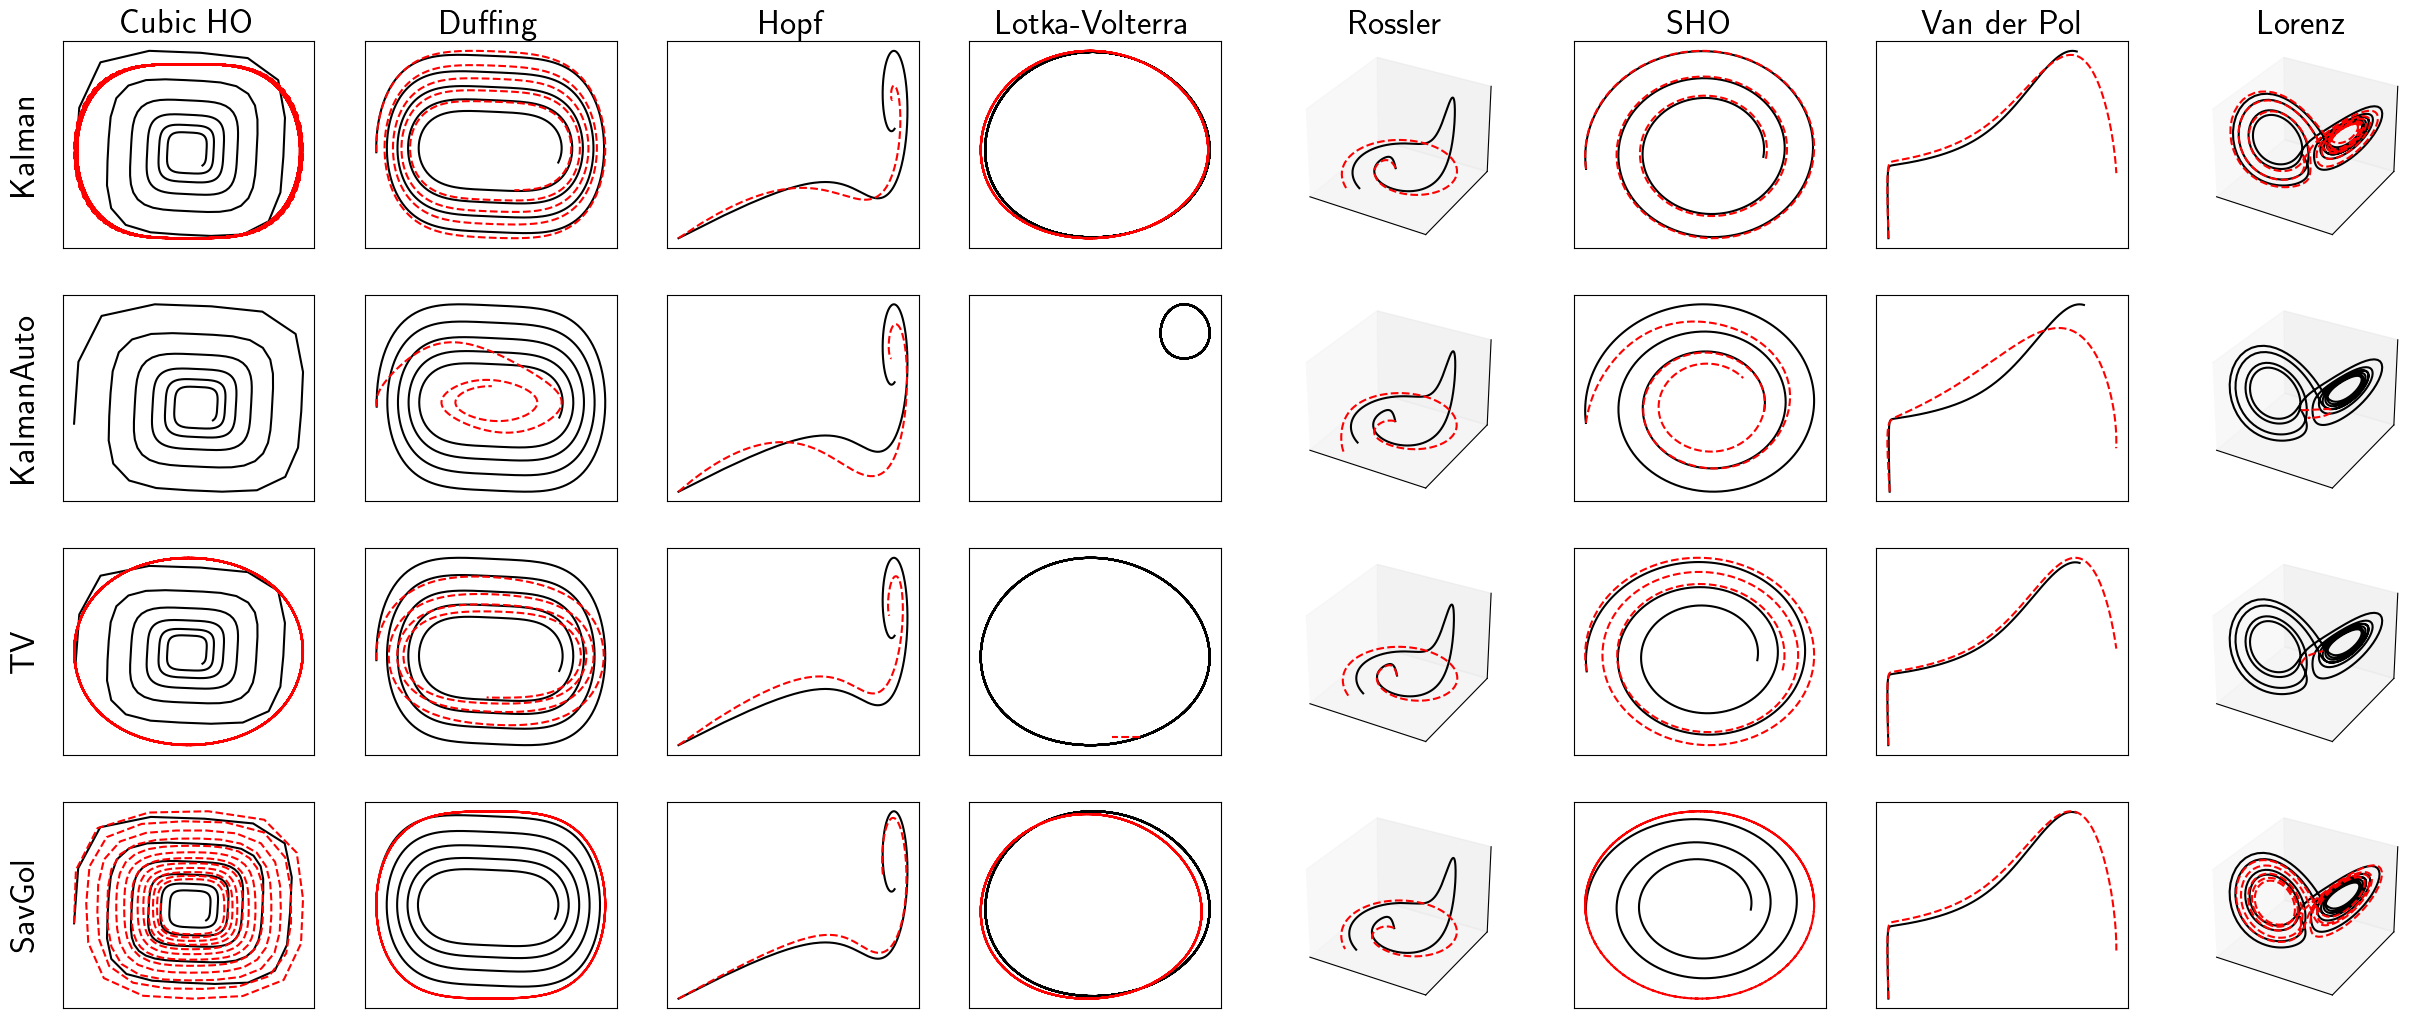
\includegraphics[height=\pdfpageheight]{images/summary_test}
\end{figure}
\begin{figure}
    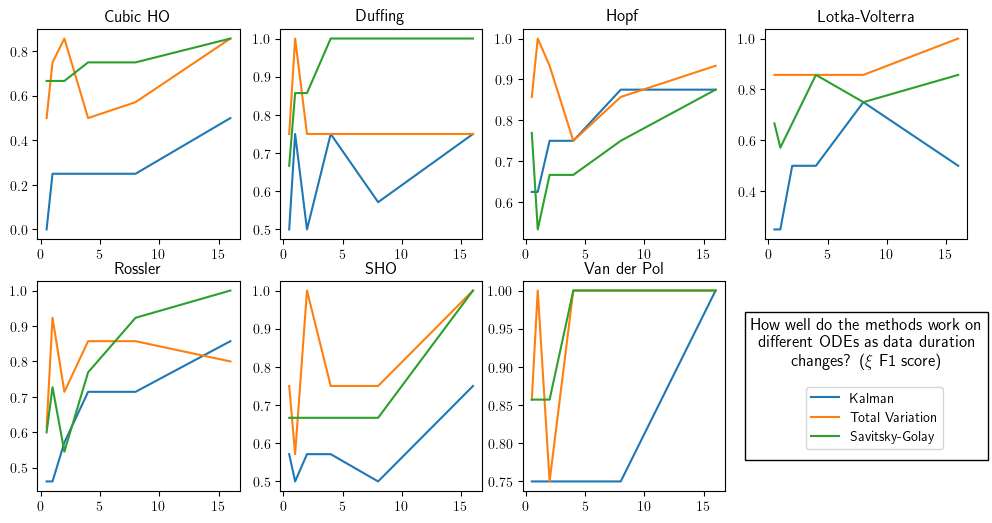
\includegraphics[width=\textwidth]{images/summary_f1}
\end{figure}
\begin{figure}
    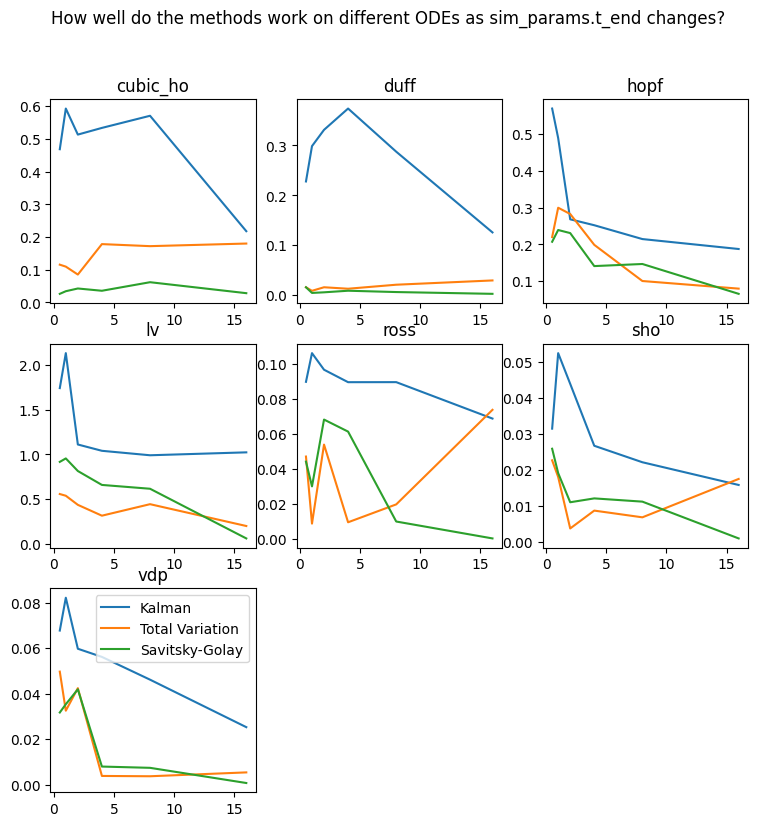
\includegraphics[width=\textwidth]{images/summary_mae}
\end{figure}
% Methods:
% \begin{itemize}
%     \item table
%     \item Compare with (a) WeakSINDy, (b) TV, SG filter
%     \item metrics: F1, MAE of coefficients (\textcolor{red}{or MSE?})
%     \item Utilize MIOSR optimizer (\textcolor{red}{with Ensembling wrapper?})
% \end{itemize}
% ODE data sets \textcolor{red}{Do I add {\it all} the possible ones I have set up (Rossler, Duffing)?  Do I add the reaction network one?}
% \begin{itemize}
%     \item Hudson Bay Company Lotka-Volterra
%     \item Van der Pol oscillator
%     \item Hopf
%     \item MHD \textcolor{red}{Would need to add}
% \end{itemize}
% PDE Data sets \textcolor{red}{anything real?}
% \begin{itemize}
%     \item Inviscid Burgers
%     \item KdV
%     \item nonlinear Schrodinger
%     \item KS
%     \item Reaction-Diffusion
% \end{itemize}

% \subsection{Noise tolerance and data length}
% \textcolor{blue}{Figure: plot of score for each method across range of smoothing parameters.  subplots for each ODE \& metric}.  \textcolor{red}{Parameter-search wrapper-experiment inside P-search comparison experiment}.
% % \subsection{ODEs: Robust Kalman Smoothing (Maybe?)}
% \textcolor{blue}{Figure: plot of score for each method across range of smoothing parameters.  subplots for each ODE \& metric}. 
% Add noisy 
% \subsection{ODEs: Data Length requirements}
% \textcolor{blue}{Figure: plot of score for each method at optimal parameter across range of data length requirements.  subplots for each ODE \& metric}.  \textcolor{red}{Parameter-search wrapper-experiment inside data-length wrapper-experiment inside Data-length comparison comparison experiment}.
% \subsection{PDEs}
% \textcolor{red}{Use Figure 4 from the E-SINDy paper. Need to implement these}
% % \subsection{Model Predictive Control}
% % \textcolor{red}{Lorenz stabilization, learn from E-SINDy paper}
\section{Conclusion}
This paper has demonstrated that Kalman smoothing is a useful addition to SINDy.  By incorporating hyperparameter optimization, it makes the method more generally applicable across domains. The Kalman smoother behaves optimally for the simplest systems and provides a familiar process to the controls engineering community, even if it is not a mathematically unique innovation.  It also appears to perform better at preserving global system structure in simulation.

<More specific experimental results summary>

Since Kalman smoothing and SINDy regression loss terms accomodate variable timesteps, a natural innovation is to combinine the two into a single optimization problem.  This could allow interaction and a more clear tradeoff between fitting the data through either the smoothed process or the coefficient sparsity.

Currently, the hyperparameter optimization has no access to the terms in the SINDy expression and therefore no intrinsic understanding of the process variance even when measurement noise is known.  With access however to the library terms, hyperparameters for process and measurement variance could be more quickly selected, rather than the long prox-gradient method of \red{Boyd/Barratt}.

Kalman SINDy could also be more directly compared to Weak SINDy, which aims at the same goal of reducing the sensitivity to noise.

Oh wait, did I forget to mention that KS has a natural connection between 
% \begin{table}
%     \centering
%     \begin{tabular}{c|c}
%          &  \\
%          & 
%     \end{tabular}
%     \caption{Caption}
%     \label{tab:my_label}
% \end{table}
\end{document}
